\chapter{Background}
\label{chap:background}

\Ac{io} devices interact with the \acs{cpu} via three types of communication
primitives: interrupts, registers and shared memory. The specific design of
these primitives depends on the technologies used; we provide an overview of
device-to-host and host-to-device communication in the following sections,
focusing on \acs{pcie}, \acs{dma} and \acsp{iommu} in the context of
(high-speed) network environments. The knowledgeable reader may skip ahead to
the description of our software implementations (\Cref{chap:implementations}) or
our performance analysis of \acp{iommu} (\Cref{chap:performance_analysis}).


\section{Overview}
\label{sec:overview}

\begin{figure}[!b]
    \centering
    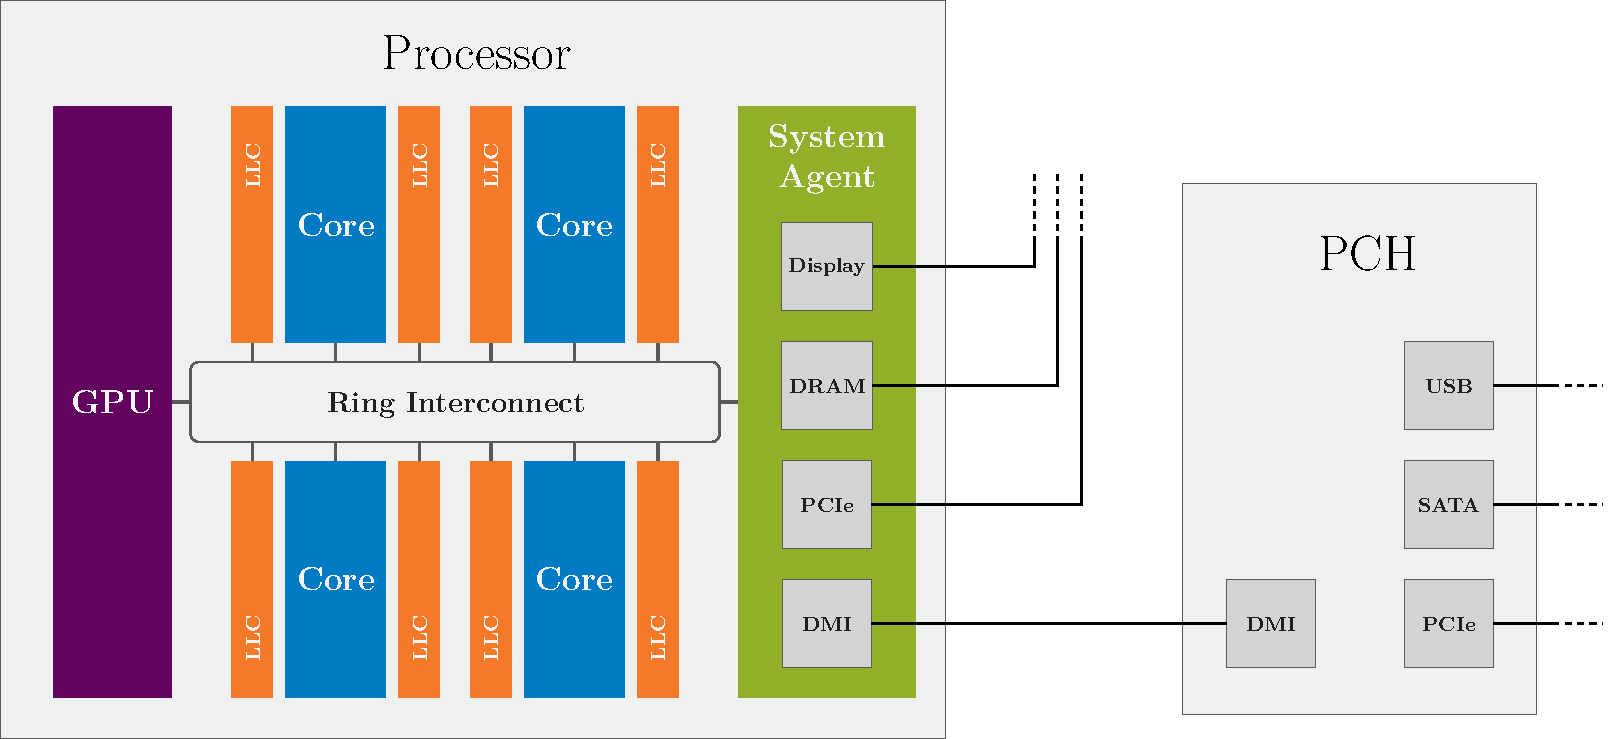
\includegraphics[width=0.8\textwidth]{figures/cpu-and-pch}
    \caption{Processor and Platform Controller Hub (PCH) on an Intel system.}
    \label{fig:pch}
\end{figure}

On modern systems, peripherals, processor and main memory are interconnected
with each other via a wide set of connection standards and protocols. Devices
are either directly attached to the \ac{cpu} via \ac{pcie} or to an \acs{io} hub
known as Platform Controller Hub~(Intel) or chipset~(AMD). Direct connections
are preferred for \ac{io} devices with high performance requirements such as
video cards or NVMe controllers. On enterprise hardware, e.g., servers, most if
not all \ac{pcie} devices are directly attached to the \ac{cpu}, whereas the
\ac{io} hub is connected to slower peripherals like on-board Gigabit network
cards or USB 2.0 ports. On consumer hardware, more devices might be attached to
the \ac{io} hub. The \ac{io} hub resides on a separate chip and is connected to
the \ac{cpu} via Direct Media Interface (Intel) or Unified Media Interface
(AMD). \Cref{fig:pch} illustrates the relationship between \ac{cpu}, \ac{io} hub
and peripherals.

Conceptually, system agent and Platform Controller Hub (PCH) depicted in
\Cref{fig:pch} are successors of northbridge and southbridge from previous
chipsets. While memory controller and other northbridge functions were
incorporated into the \ac{cpu} as so-called system agent, southbridge and
remaining northbridge functions were moved to the PCH.


\section{PCI Express}
\label{sec:pcie}

As de-facto standard, \acf{pcie} is used for communication with most
peripherals. \ac{pcie} is a high-speed serial bus that was designed to replace
PCI and PCI-X. Unlike the former, \ac{pcie} is based on a point-to-point
topology and encapsulates all communication data in \ac{pcie} packets.
Additionally, \ac{pcie} supports hotplugging of devices. Similar to other
network protocols, \ac{pcie} consists of various communication layers,
acknowledgements and flow control for reliable data transmission.

Physically, \ac{pcie} devices are connected via lanes which consist of two
differential pairs each, i.e., four wires per lane. The two pairs of \ac{pcie}
lanes are used unidirectionally as transmit / receive channels. Together, they
form a bidirectional link. For interrupts, no physical pin is used. Instead,
in-band messages signal interrupts to the interrupt controller which interrupts
the \ac{cpu}.

\begin{figure}[!b]
    \centering
    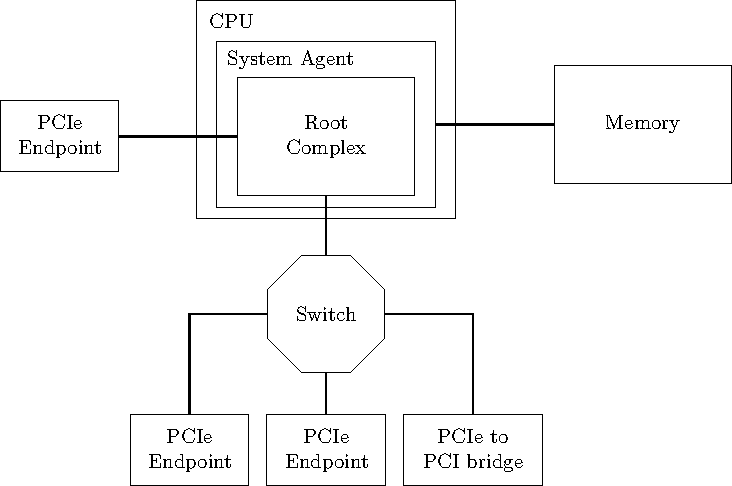
\includegraphics[width=0.6\textwidth]{figures/pcie-tree}
    \caption{Exemplary \acs{pcie} topology on an Intel system.}
    \label{fig:pcie-topology}
\end{figure}

Devices may use up to 32 lanes to increase throughput. Transfer rates of the
lanes have stepped up by a factor of ten since \ac{pcie} 1.0: Today's commonly
used \ac{pcie} 4.0 (which was released in 2017) yields a serial data rate of 16
Gbps per lane which corresponds to about 1.97 GB/s taking the 128b/130b line
code into account.

\ac{pcie} devices and processor are connected through switches.
\Cref{fig:pcie-topology} depicts a typical \ac{pcie} tree. On the \ac{cpu} side,
connections end in the \ac{pcie} root complex which is part of the system agent
on Intel systems and the bridge between \ac{cpu}, main memory and devices. On
the device side, connections end at \ac{pcie} endpoints. \ac{pcie} devices may
initiate transfers to main memory through the \ac{pcie} root complex, acting as
\acs{dma} bus masters that access main memory independently of the \ac{cpu}.

\ac{pcie} uses three layers for communication: physical layer, data link layer
and transaction layer. The physical layer of \ac{pcie} is responsible for link
initialization and point-to-point data transfer. The data link layer ensures
reliable transport of data between individual \ac{pcie} endpoints, or endpoints
and the root complex. The transaction layer contains user application data or
configuration data for the link, and routing information like transmitter and
receiver IDs for memory or \ac{io} requests.

Every \ac{pcie} transmission consists of four bytes that mark the start of a new
packet, a header of 12 bytes (or 16 when using 64 bit addresses), a payload of
up to 4,096 bytes (depending on the maximum payload size on the link), and four
to eight bytes of packet checksums. Thus, minimal packet overhead for headers,
checksums, etc. is 20 bytes.

\ac{pcie} packets are categorised into requests and completions. Requests are
memory, \ac{io} or configuration reads and writes (to the PCI configuration
space) that are either posted or non-posted, i.e., expect a completion (reply)
or not. The PCI configuration space is a standardized register space that
contains information about a PCI(e) device such as vendor and device ID, device
class or the physical addresses of the device's registers (i.e., the Base
Address Registers or BARs). Among others, memory space is used by a device to
access main memory and by the \ac{cpu} to access device registers. \ac{io} space
is included for backwards compatibility and will probably be deprecated in the
future.

Device registers can be accessed via memory-mapped \ac{io} or port-mapped
\ac{io}. With memory-mapped \ac{io}, main memory and \ac{io} share the same
address space, i.e., addresses refer to devices and main memory. With
port-mapped \ac{io}, special \ac{cpu} instructions and an \ac{io} pin on the
\ac{cpu} or a separate \ac{io} bus to perform \ac{io} are used.

To access the configuration space of \ac{pcie} devices, addresses consisting of
an eight bit bus number, five bit device number and three bit function number
are used (commonly referred to as BDF, i.e., bus/device/function). See
\Cref{fig:pcie-bdf} for reference.

\begin{figure}
    \centering
    \begin{bytefield}[endianness=big,bitwidth=0.03\linewidth]{16}
        \bitheader{0-15} \\
        \bitbox{8}{Bus \#} & \bitbox{5}{Device \#} & \bitbox{3}{Fn \#}
    \end{bytefield}
    \caption{\acs{pcie} IDs as bus/device/function triple.}
    \label{fig:pcie-bdf}
\end{figure}

On system boot, every \ac{pcie} root complex is enumerated to determine which
slots have devices installed. During enumeration, BIOS or \ac{os} probe the
\ac{pcie} configuration space for all possible combinations of bus and device
number, i.e., by reading vendor and device ID of \ac{pcie} switches and
endpoints. It suffices to probe for function 0 for every combination of bus and
device number to determine a device's presence since every device is required to
implement function 0. For every detected device, the maximum payload size on the
link is determined and the device is assigned its respective BDF. Bus and device
numbers might be re-assigned by the enumeration software if a \ac{pcie} device
is hotplugged.

After a device's presence has been detected, every base address register field
in the configuration space is read to determine the address space needed to
access the registers of the device and subsequently every device is assigned a
portion of the host physical address space. If software sets one of the device's
registers through memory-mapped \ac{io}, e.g., during device setup by a device
driver, a memory write to the physical address is issued. The \ac{pcie} root
complex -- which unites the physical address space of all its devices --
receives the memory write, translates the physical address to the BDF of the
respective device and initiates a \ac{pcie} memory write transaction to the
device.


\section{Network Interface Controllers}
\label{sec:nics}

A very common kind of \ac{pcie} peripherals are network cards used for
communication between computer systems via wireless (e.g., WLAN) or wired (e.g.,
LAN) networks, often connecting hosts via a gateway to the Internet. Another
term for network cards is \acfp{nic}.

\begin{figure}[!b]
    \centering
    \includegraphics[width=0.4\textwidth]{figures/tx-ring}
    \caption{TX descriptor ring of a Network Interface Controller.}
    \label{fig:tx-ring}
\end{figure}

Various manufacturers produce a wide range of \acp{nic} for various
applications, be it for data centers with special performance requirements or
for the consumer sector. As versatile as these \acp{nic} are, so are the drivers
used for their operation, and complexity of drivers and devices increases
steadily: whereas early \acp{nic} were merely capable of receiving and
transmitting network packets, modern network cards offer huge amounts of
(hardware-offloading) features like checksum calculations, encryption and
authentication of packets, VLAN tagging and flow control, time syncing, traffic
shaping, etc.

This complexity is reflected in several ways: On the one hand in manuals (the
datasheet for network cards of the Intel 82599 family \cite{intel2016datasheet}
consists of more than 1,000 pages) and drivers (exceeding 100,000 lines of code
for some devices \cite{emmerich2019case}). On the other hand in devices like
Intel's XL710 which follows a more firmware-driven design where much
functionality is executed on the network card, and driver and \ac{nic}
communicate via a message based interface \cite{emmerich2019user}. The downside
of this development is a lack of reliability, safety and security in computer
systems: in case of Linux, 39 out of 40 memory bugs found in the kernel in 2017
were located in device drivers \cite{emmerich2019case}.

Although \acp{nic} have changed a lot in the last decades, most of them still
use a seemingly simplistic interface to communicate reception or transmittal of
packets: descriptor rings. Descriptor rings are circular buffers that contain
information about network packets and are shared between \ac{nic} and host.
\acp{nic} that use descriptor rings have RX and TX descriptor rings.
\Cref{fig:tx-ring} shows a TX descriptor ring. Descriptors in TX descriptor
rings describe outgoing packets, i.e., the amount of data to be sent, location
in memory (e.g., of buffers in a memory pool), whether transmittal of the packet
should be reported by the \ac{nic} through updating its descriptor, etc.
Conversely, descriptors in RX descriptor rings describe where incoming packets
can be stored by the \ac{nic}.

Ownership of descriptor rings is shared between \ac{nic} and host through two
queue pointers, a head and a tail pointer. In case of the TX descriptor ring,
the \ac{nic} manages the head pointer (TDH) while the device driver manages the
tail pointer (TDT). At device initialization, head and tail pointer are set to
the first descriptor. Once a packet is queued by the driver, i.e., the
descriptor in the TX descriptor ring has been changed appropriately, the driver
updates the tail pointer to the next descriptor, thereby transfering ownership
of all descriptors between head and tail pointer to the \ac{nic}. Conversely,
the \ac{nic} updates the head pointer once a descriptor was processed and the
corresponding packet data has been fetched from main memory by the \ac{nic}.

If the tail pointer points to the descriptor preceding the head pointer's
descriptor, the TX queue is full and no new data can be queued for transmittal.
Consequently, the driver has to wait until some packets have been sent out by
the \ac{nic}.


\section{Direct Memory Access}
\label{sec:dma}

Access to main memory by hardware without \ac{cpu} involvement is known as
\acf{dma}. In multi-core processors, \ac{dma} is sometimes used to transfer data
between cores. In conjunction with \ac{pcie} devices, \ac{dma} is performed
through \ac{pcie} memory read and write transactions. With \ac{pcie}, no
separate \ac{dma} controller is used (third-party DMA), instead reads and writes
are issued directly from bus masters (first-party DMA), i.e., \ac{pcie} devices
allowed to read/write memory or \ac{io} space, to the root complex and
subsequently to main memory via the memory controller. For ordinary \ac{dma},
physical addresses are used to access main memory, just as they are used by the
\ac{cpu} when accessing device registers through memory-mapped \ac{io}.

Using physical addresses is disadvantageous as \ac{pcie} devices may read from
and write to any memory address of main memory. This is a problem for

\begin{itemize}
    \item device pass-through to virtual machines, since virtual machines might
        read host memory outside of their access range through the memory
        accessing capabilities of \ac{pcie} devices;
    \item legacy 32-bit devices on 64-bit hosts, since they cannot access memory
        outside of their address space -- i.e., the first 4 GiB of host physical
        address space -- without bounce buffers and expensive memory copying by
        the \ac{os};
    \item avoiding harm from malicious or faulty drivers, since secrets can be
        read from main memory and \ac{os} data structures can be corrupted;
    \item avoiding harm from malicious or faulty devices;
    \item providing secure unprivileged access to hardware, e.g., in case of
        user-space network drivers.
\end{itemize}

To solve these problems, virtual addresses are used for \ac{io} devices on
modern computer systems instead of physical addresses. Similar to process
virtual addresses and \acp{mmu}, \ac{io} virtual addresses (IOVAs) are assigned
to devices and a translation unit is inserted into the data path that restricts
memory accesses to a device's memory region. Such translation units are commonly
known as \acfp{iommu}.


\section{Input-Output Memory Management Units}
\label{sec:iommus}

\acp{iommu} are multipurpose devices that virtualize the memory space of
peripherals. Although there is a trend to use \acp{iommu} as a protection
mechanism against malicious or faulty peripherals, the primary application for
\acp{iommu} is and remains virtualization, i.e., direct pass-through of \ac{io}
devices to virtual machines for performance reasons.

Conceptually, \acp{iommu} may be used for any kind of \ac{io} devices and any
kind of connection standards. In practice, \acp{iommu} are implemented in the
\ac{pcie} root complex since in today's systems almost all if not all \ac{io}
devices are connected to the \ac{cpu} via the \ac{pcie} root complex: modern
interfaces like Thunderbolt, NVMe and SATA Express are directly built on top of
\ac{pcie}, whereas for older connection standards like USB or I$^2$C, \ac{pcie}
hubs are used. Focus of \acp{iommu} on \ac{pcie} is also reflected in code like
Linux's \ac{iommu} API that is closely centered around \ac{pcie} instead of
providing an abstract interface for any kind of \ac{io} devices and connections.

\begin{figure}
    \centering
    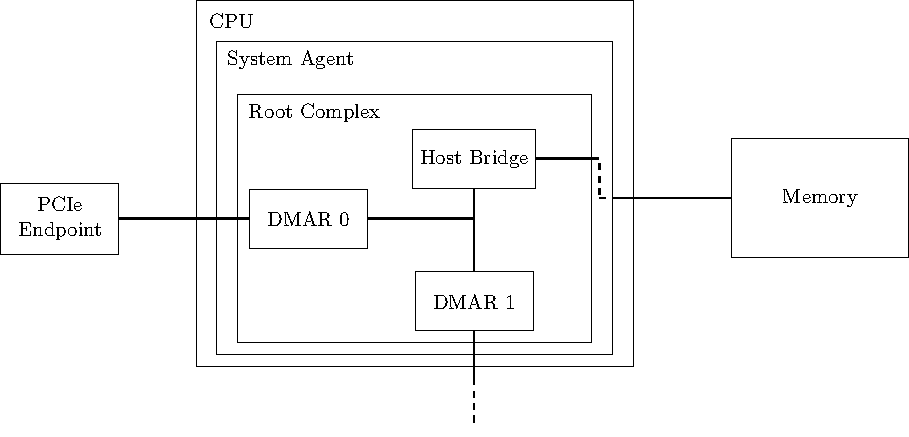
\includegraphics[width=0.7\textwidth]{figures/pcie-dmar}
    \caption{DMAR units in the PCIe root complex of an Intel system.}
    \label{fig:pcie-dmar}
\end{figure}

The main task of \acp{iommu}, which is filtering requests and address
translation, is performed by so-called \ac{dma} remapping (DMAR) hardware units:
When \ac{io} devices attempt to access main memory, the request is intercepted
by the DMAR unit, checked for admissibility and translated appropriately. This
procedure consists of two major steps: First, a device's domain is determined by
it's bus/device/function (BDF) number. Second, the domain's translation tables
are consulted to map the requested address to a host physical address.

A \ac{pcie} root complex may contain one or multiple \acp{iommu} where each DMAR
is responsible for a distinct set of \ac{io} buses (\Cref{fig:pcie-dmar}).
Devices on \ac{iommu}-managed buses belong to protection domains, i.e., sets of
address mappings and access permissions. While domains may consist of multiple
devices, devices cannot be assigned to multiple domains (i.e., every device is
mapped to exactly one domain).

Data structures used for address translation by the DMARs are kept in main
memory to be accessible for \ac{os} and \acp{iommu}. In case of multiple
\acp{iommu}, DMARs may share the same data structures. On \ac{iommu}
initialization, the \ac{os} sets up these data structures by creating domains
and address mappings for the system's \ac{io} devices. Although this happens
during system boot, mappings are not fixed: the device-to-domain mapping may
change (e.g., when a device is assigned to a virtual machine) and address
mappings may be altered by the \ac{os} (e.g., when \ac{dma} memory is mapped or
unmapped).

Depending on the usage model of the \ac{iommu}, addresses used by \ac{io}
devices may be one of the following:

\begin{itemize}
    \item I/O virtual addresses (IOVAs) managed by software on the host,
    \item guest I/O virtual addresses managed by software in a virtual
        machine,
    \item guest physical addresses of a virtual machine,
    \item guest virtual addresses of software running in a virtual machine.
\end{itemize}

\begin{figure}[!b]
    \centering
    \includegraphics[width=1.0\textwidth]{figures/iova-translation}
    \caption{Intel \acs{iommu} address translation of 48-bit addresses to 4~KiB
    pages. Adapted from \textit{IOMMU protection against I/O attacks: a
    vulnerability and a proof of concept} \cite{morgan2018iommu}.}
    \label{fig:translation}
\end{figure}

For different address types, hardware implementations of \acp{iommu} may support
different translation schemes. In case of virtualization, \acp{iommu} may be
used for nested translation of addresses: a first-level translation to translate
a guest virtual address to a guest physical address, followed by a second-level
translation translating the guest physical address to the host physical address.

\Cref{fig:translation} depicts the single-level translation mechanism of an
Intel \ac{iommu} for 48-bit IOVA addresses to 4 KiB pages. After an attempt to
read or write main memory has been intercepted by the \ac{iommu}, the first
table to be consulted -- if translation was enabled in the global command
register of the \ac{iommu} -- is the root table. The physical address of the
root table is stored in the Root Table Address Register (RTAR) of the
\ac{iommu}. The root table consists of 256 root entries 16~B each, i.e., 4~KiB
in total. Every root entry has a bit that indicates presence of a context table
for this entry. The root table is indexed by the bus number of the device and --
in conjunction with device and function number -- determines the context entry
for this device.

Like the root table, the context table is a 4~KiB page with 256 16~B entries.
Every context entry represents an IOMMU domain. Context entries contain a field
indicating whether requests belonging to this domain may pass the \ac{iommu}
untranslated, and -- in the more likely case that addresses must be translated
-- a pointer to the first table to be used for address translation for this
domain, the PML4 table.

Subsequently, PML4, PDP, PD and PT table are walked by the \ac{iommu} to
determine the host physical address belonging to the IOVA address. Every table
is a 4~KiB page with 512 8~B entries. If there is no translation for a requested
address or the access rights for associated page do not permit access,
translation faults and the request is rejected.

In case of 2~MiB pages, no PT table is used for translation, and the last
21~bits of the IOVA address represent the offset into the 2~MiB page. In case of
1~GiB pages, no PT and no PD table are used, and the last 30~bits of the IOVA
address represent the offset into the 1~GiB page.

PML4, PDP, PD and PT table form a 4-level translation structure. For 57-bit IOVA
addresses, a 5-level structure is used with an additional PML5 table. For 39-bit
IOVA addresses, a 3-level structure is used.

To speed up address translation, \acp{iommu} cache translation information in a
context cache and a \ac{tlb}, the \ac{iotlb}. Context cache and \ac{iotlb}
increase performance but also complexity: Caches have to be kept up-to-date and
entries must be purged from the caches when they become invalid, necessitating
some kind of invalidation mechanism.


\section{IOMMUs on Linux}
\label{sec:iommus_on_linux}

Linux supports \acp{iommu} of all major vendors: besides Intel and AMD, the
kernel also includes drivers for \acp{iommu} from ARM, Qualcomm, Texas
Instruments, Samsung, Nvidia, IBM and other, less well-known manufacturers.

\acp{iommu} are not used by default on all architectures. In case of Intel x86,
Linux ignores any DMAR units and enables its own software \ac{iommu} called
SWIOTLB. The SWIOTLB is more of a poor man's \ac{iommu} that uses bounce
buffers: At boot time, a contiguous chunk of memory (usually 64~MBs) is reserved
in the lower address space of main memory and used for \ac{dma}-capable devices
with limited addressing capabilities, e.g., legacy 32-bit devices. When an
already allocated DMA buffer is to be used by a device that cannot address the
buffer directly, memory in the lower address space, the so-called aperture, is
linked to that buffer, passed to the device, and data is copied back and forth
by the \ac{os} between the device-used memory in the aperture and the
device-inaccessible buffer.

On AMD systems, \acp{iommu} are enabled by default. For Intel, this behavior can
be enforced through a kernel boot parameter. When \acp{iommu} are enabled, Linux
checks the ACPI tables of BIOS/UEFI for DMARs on system boot. For every DMA
Remapping Hardware Unit Definition (DRHD) in the DMA remapping (DMAR) reporting
ACPI tables, Linux initializes the DMAR unit through its respective device
driver, creates a default \ac{iommu} domain and assigns all \ac{pcie} devices to
\ac{iommu} groups, where each group represents the smallest possible set of
devices that can be distinguished by the \ac{iommu} (e.g., all devices behind a
PCI bridge belong to the same group). Furthermore, each \ac{iommu} group is
assigned to an \ac{iommu} domain.

Linux has a number of kernel boot parameters to change its default behavior in
relation to \acp{iommu}. (SW-)\acp{iommu} can be disabled or enforced, the
default domain can be set to pass-through so that devices bypass the \ac{iommu}
if not specified otherwise, and depending on the driver, the policy of
\ac{iotlb} management can be changed as Linux defers \ac{iotlb} invalidation by
default which increases performance but creates a window for invalid \ac{dma}
accesses, i.e., devices may access some \ac{dma}-able memory that has been
unmapped already as requests are still translated by the \ac{iotlb}. For the
Intel \ac{iommu}, \ac{iotlb} invalidation can be set to strict mode to enforce
immediate flushing of the \ac{iotlb}. The AMD \ac{iommu} driver provides a
similar option called \texttt{fullflush}. If no deviating behavior was
requested, Linux flushes the \acp{iotlb} every 10 ms or every 256 batched
invalidation requests.

While all \acp{iommu} are managed by its respective device drivers, other kernel
drivers implicitely change the \ac{iommu} configuration through Linux's
\ac{dma}-API by allocating, mapping and unmapping \ac{dma} memory, enforcing
action by the driver depending on the operation and settings (e.g., immediate
flushing of all \acp{iotlb} by the \ac{iommu} driver).

For controlled device access in user-space, e.g., by user-space network drivers,
Linux offers a framework called Virtual Function I/O (VFIO). The framework
consists of a device driver and various methods to interact with
\ac{iommu}-controlled \ac{pcie} devices.

Devices to be used through VFIO have to be bound to the VFIO device driver. If a
device's group contains multiple devices, all have to be bound to the driver or
must be unbound from other host drivers (which will make the group available
except the unbound devices). Device groups successfully bound to the VFIO driver
appear as files in Linux's device filesystem at \linebreak
\texttt{/dev/vfio/\{group-number\}}. By chowning a device's group file to the
current user, unprivileged access to the \ac{pcie} devices of the group is
granted in a safe manner.

In VFIO, every \ac{iommu} group in use belongs to a container. Depending on the
\ac{iommu} driver's capabilities, one or multiple groups may be encapsulated
into a container, and containers may contain groups of different \ac{iommu}
domains.

To access a VFIO-bound device in user-space, multiple steps have to be carried
out by an application. First, a VFIO container is created and initialized for
the device to be used or an existing container is re-used. Second, the device's
group file is opened by the user-space application and the group is added to the
VFIO container. Third, a file descriptor to the device is derived through a VFIO
method on the group file. Fourth, the device file descriptor is used to map the
device's registers into virtual memory. Finally, memory for \ac{dma} operations
may be allocated in user-space and \ac{iommu} mappings to that memory may be
created through the VFIO-API, returning IOVA addresses that can be passed to the
device.


\section{Single-Root Input/Output Virtualization}
\label{sec:sriov}

Single-root input/output virtualization is a mechanism that allows a \ac{pcie}
device to appear as multiple devices and thus be shared with multiple virtual
machines. Devices that support SR-IOV report this ability to the host through
their PCI configuration space which includes registers for SR-IOV Extended
Capability.

When SR-IOV is enabled for a device, the device can be split into a physical
(PF) and multiple virtual functions (VFs). The PF is the standard \ac{pcie}
function of the device which has full control over the device, is used to reset
and initialize it and to enable and disable VFs. Hence, access to the physical
function is usually restricted to \ac{os}. VFs on the other hand only support a
subset of device operations, primarily to manage packet receival and transmittal
of the function, and can be passed to virtual machines in a safe manner.

For virtual functions, slightly different drivers have to be used as virtual
functions use different device registers and have to communicate with the
physical function driver for certain operations like reset of the VF. A physical
function driver on the other hand must be able to handle these requests and is
therefore slightly more complex than the same driver without SR-IOV support.

On Linux, virtual functions of SR-IOV-capable devices can be created when
loading the PF kernel driver, e.g., in case of \texttt{ixgbe}: \texttt{modprobe
ixgbe max\_vfs=2}, which results in the PF driver creating two virtual functions
for every \texttt{ixgbe}-bound device in the system, or by writing the required
number of virtual functions into a device \texttt{sysfs} file called
\texttt{sriov\_numvfs}.

When VFs are created by the PF driver, every VF is assigned a \ac{pcie}-BDF
triple such that the virtual function can be adressed directly and identified on
the \ac{pcie} bus. Usually, the PF also assigns MAC addresses to the VFs and
configures the \ac{nic} such that each VF receives the packets destined to its
MAC address. To prevent MAC address spoofing, outgoing packets must be sent from
the VF's MAC address and are dropped by the \ac{nic} in case VFs do not comply.
The MAC anti-spoofing mechanism can be disabled by the PF driver.

While not required, SR-IOV can be used in conjunction with \acp{iommu} to pass
VFs safely to virtual machines. When devices are passed-through without
\acp{iommu}, virtual machines have unlimited access to the machine's main memory
through the virtual function (see \Cref{sec:dma}).

